\begin{definition}
Allgemein ist die Aufgabenstellung der Optimierung wie folgt
definiert:
\begin{equation}
  \min_{x \in \F} f(x) \tag{P} \label{prob:allg_opt_prob}
\end{equation}
Die Funktion $f \colon D \subseteq \R^n \rightarrow \R$ ist die sogenannte
Zielfunktion.
$D$ sei der Definitionsbereich von $f$.
$\F$ sei eine nichtleere Teilmenge von $D$, die man als L�sungsmenge bezeichnet.
Alle Elemente von $\F$ werden als zul�ssige Punkte bezeichnet.
$\F$ wird durch die sogenannten Nebenbedingungen oder Restriktionen definiert.
\end{definition}

Falls $\F = D$ gilt,
bezeichnet man das Optimierungsproblem als unrestringiert.
Es besitzt also keine Restriktionen.
Ansonsten hei�t es restringiertes Optimierungsproblem.

In der Regel definiert man ein Optimierungsproblem als Minimierungsproblem,
weil ein Maximierungsproblem $\max g(x)$ zum Minimierungsproblem
$\min f(x) := -g(x)$ �quivalent ist.

\begin{definition}
\emph{(Globale und lokale L�sung, vgl. Definition 1.1.4 in
\cite[S.~2~f.]{alt})}\\
Ein Punkt $\xopt \in \F$ hei�t globale L�sung des Problems~\eqref{prob:allg_opt_prob} oder
globales Minimum, wenn
\begin{equation}
  f(\xopt) \leq f(x) \qquad \forall x \in \F
\end{equation}
gilt.
Ein Punkt $\xopt \in \F$ hei�t strikte globale L�sung des Problems~\eqref{prob:allg_opt_prob} oder
striktes globales Minimum, wenn
\begin{equation}
  f(\xopt) < f(x) \qquad \forall x \in \F\backslash\{\xopt\}
\end{equation}
gilt.
Ein Punkt $\xopt \in \F$ hei�t lokale L�sung des Problems~\eqref{prob:allg_opt_prob} oder
lokales Minimum, wenn f�r eine Umgebung $U(\xopt)$ von $\xopt$
\begin{equation}
  f(\xopt) \leq f(x) \qquad \forall x \in U(\xopt) \cap \F
\end{equation}
gilt.
Ein Punkt $\xopt \in \F$ hei�t strikte lokale L�sung des Problems~\eqref{prob:allg_opt_prob}
oder striktes lokales Minimum, wenn f�r eine Umgebung $U(\xopt)$ von
$\xopt$
\begin{equation}
  f(\xopt) < f(x) \qquad \forall x \in U(\xopt) \cap \F\backslash\{\xopt\}
\end{equation}
gilt.
Eine Umgebung $U(\xopt)$ von $\xopt$ ist eine offene Menge, die $\xopt$
beinhaltet.
\end{definition}

Von diesen Definitionen kommt der Begriff \emph{globale Optimierung} her.
Bei der globalen Optimierung versucht man, eine globale L�sung zu finden.
Viele Verfahren versuchen nur lokale L�sungen zu bestimmen,
weil globale L�sungen nicht so einfach zu bestimmen sind.

\begin{example}\label{example:unrestr_opt_prob}
\emph{(Vgl. Beispiel 1.1.2 in \cite[S.~1]{alt})}\\
Ein Beispiel eines unrestringierten Optimierungsproblems ist
\begin{equation}
  \min_{x \in \R}\ f(x) := (2x-2)^2 (3x+3)^2 + 10x.
\end{equation}
Dieses Problem hat eine strikte globale L�sung an der Stelle $\xopt = -1$
und eine strikte lokale L�sung an der Stelle $x = 1$
(siehe Abbildung~\ref{fig:beispiel_unrestr_opt_prob}).
\end{example}
\begin{figure}[ht]
\centering
\begin{tikzpicture}[yscale=0.7,xscale=2.5]
  \draw[very thin,color=gray,ystep=2,xstep=0.5] (-1.47,-2.9) grid (1.47,7.4);
  \draw[->] (-1.48,0) -- (1.48,0) node [above] {$x$};
  \draw[->] (0,-3) -- (0,7.5) node [right] {$f(x)$};
  \foreach \x/\xtext in {-1,-0.5/-\frac{1}{2},0,0.5/\frac{1}{2},1}
    \draw (\x,0.1) -- (\x,-0.1) node [below,fill=white] {$\xtext$};
  \foreach \y/\ytext in {-2/-20,0,2/20,4/40,6/60}
    \draw (0.03,\y) -- (-0.03,\y) node [left,fill=white] {$\ytext$};
  \draw[color=blue] plot[smooth] file {images/beispiel-unrestr-opt-prob.table};
\end{tikzpicture}
\caption{Die Funktion von Beispiel \ref{example:unrestr_opt_prob}}
\label{fig:beispiel_unrestr_opt_prob}
\end{figure}

\begin{definition}
\emph{(Nichtlineare Optimierungsprobleme)}
Die Aufgabenstellung bei der nichtlinearen Optimierung
mit Gleichungs- und Ungleichungsrestriktionen kann man
spezifischer wie folgt definieren:
\begin{align}
  \min_{x \in D}\ & f(x) \tag{PN}\label{prob:opt_prob_mit_nichtlin_restr} \\
              \nb & g(x) \leq 0 \notag \\
                  & h(x) = 0 \notag
\end{align}
Die Zielfunktion ist wieder die Funktion
$f \colon D \subseteq \R^n \rightarrow \R$.
Die Nebenbedingungen sind von den Funktionen
$g \colon D \subseteq \R^n \rightarrow \R^p$ und
$h \colon D \subseteq \R^n \rightarrow \R^m$ abh�ngig,
d.\,h., die Menge $\F$ sieht hier so aus:
$\F = \{ x \in \R^n \,|\, g(x) \leq 0, \, h(x) = 0  \}$.
\end{definition}

Die Bezeichnung \textss{Nb.} steht hier als Abk�rzung f�r
\textss{unter der Nebenbedingung} oder \textss{unter den Nebenbedingungen}.
Die Operatoren $\leq$ und $=$ vergleichen hier die Vektoren
miteinander elementenweise.
Die Zahl $0$
ist hier, je nach dem in welchem Kontext,
ein Element von $\R$, $\R^p$ oder $\R^m$.

Man kann das Problem~\ref{prob:opt_prob_mit_nichtlin_restr}
ausf�hrlicher schreiben, indem man die Funktionen
$g$ und $h$ in skalare Funktionen $g_1, \ldots, g_p \colon \R^n \rightarrow \R$
und $h_1, \ldots, h_m \colon \R^n \rightarrow \R$ zerlegt, sodass
\begin{equation*}
  g(x) =
    \left(
    \begin{array}{c}
      g_1(x) \\
      \vdots \\
      g_p(x)
    \end{array}
    \right)
\quad \text{und} \quad
  h(x) =
    \left(
    \begin{array}{c}
      h_1(x) \\
      \vdots \\
      h_m(x)
    \end{array}
    \right).
\end{equation*}

Man bekommt dann das Problem
\begin{align*}
  \min_{x \in D}\ & f(x) \\
              \nb & g_i(x) \leq 0 \text{ f�r } i = 1,\ldots,p \\
                  & h_j(x) = 0 \text{ f�r } j = 1,\ldots,m.
\end{align*}

Man kann hierbei den Unterschied zwischen der linearen Optimierung und
der nichtlinearen Optimierung gut erkennen.
Bei der linearen Optimierung muss die Zielfunktion linear sein
(d.\,h., die Zielfunktion muss in der Form $f(x) = c^T x$, $c \in \R^n$, sein)
und die Nebenbedingungen sollen durch lineare Gleichungen bzw.
Ungleichungen definiert werden.
Bei der nichtlinearen Optimierung gibt es dagegen keine Einschr�nkung,
wie die Zielfunktion und die Nebenbedingungen aussehen sollen.

\begin{example}\label{example:opt_prob_mit_nichtlin_restr}
\emph{(Vgl. Problem 1.2 in \cite[S.~3]{nocedal})}\\
Ein Beispiel eines restringierten Optimierungsproblems ist
\begin{equation}
\begin{split}
  \min_{x \in \R^2}\ (x_1-2)^2 & + (x_2-1)^2 \\
  \nb x_1 + x_2 & \leq 2 \\
          x_1^2 & \leq x_2.
\end{split}
\end{equation}
Die Abbildung~\ref{fig:beispiel_opt_prob_mit_nichtlin_restr}
zeigt die zul�ssige Menge $\F$,
die H�henlinien der Zielfunktion und
die optimale L�sung~$\xopt$.
\end{example}

Eine H�henlinie ist eine Menge von Punkten,
wo die Zielfunktion einen konstanten Wert annimmt.
In Abbildung~\ref{fig:beispiel_opt_prob_mit_nichtlin_restr}
sind die H�henlinien in Form von Kreisen zu sehen
und je gr��er der Kreis ist,
desto gr��er ist der Wert der Zielfunktion.
\begin{figure}[h]
\centering
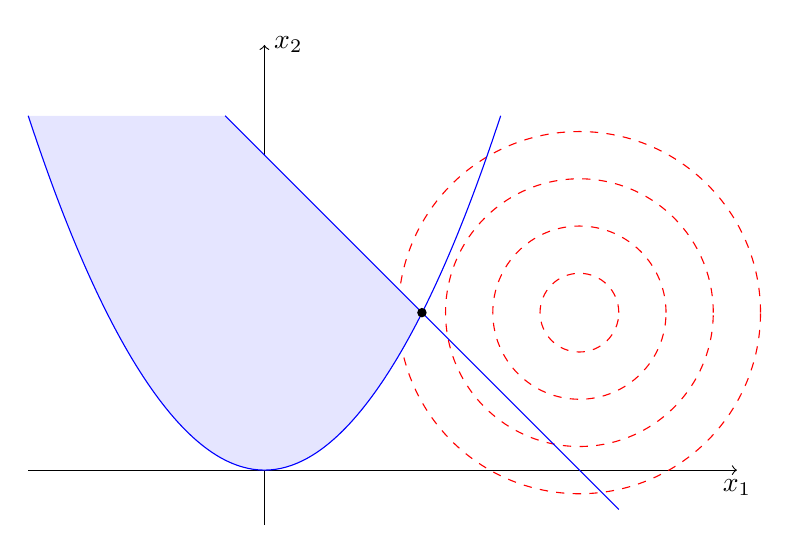
\begin{tikzpicture}[scale=2]
  \draw[->] (-1.5,0) -- (3,0) node [below] {$x_1$};
  \draw[->] (0,-0.35) -- (0,2.7) node [right] {$x_2$};
  % Die H�henlinien
  \foreach \r in {0.25, 0.55, 0.85, 1.15}
    \draw[dashed,color=red] (2,1) circle (\r);
  % Schreibe x*
  \draw (1.02,1.05) node[right,fill=white] {$\xopt$};
  % Die zul�ssige Menge F
  \fill[blue!10] (0,0) parabola (-1.5,2.25)
    (0,0) parabola (1,1) -- (-0.25,2.25) -- (-1.5,2.25);
  \draw (0,1) node {$\F$};
  % Die Nebenbedingungen
  \draw[color=blue] (0,0) parabola (-1.5,2.25) (0,0) parabola (1.5,2.25);
  \draw[color=blue] (-0.25,2.25) -- (2.25,-0.25);
  % Der Kreis f�r x*
  \fill (1,1) circle (0.03);
\end{tikzpicture}
\caption{Geometrische Darstellung
des Beispiels~\ref{example:opt_prob_mit_nichtlin_restr}}
\label{fig:beispiel_opt_prob_mit_nichtlin_restr}
\end{figure}